\documentclass[epsfig,10pt,fullpage]{article} \addtolength{\textwidth}{1.5in}
\addtolength{\oddsidemargin}{-0.75in}
\addtolength{\topmargin}{-0.75in}
\addtolength{\textheight}{1.5in}
\addtolength{\evensidemargin}{0.75in}
\raggedbottom
\usepackage{ae,aecompl}
\usepackage{epsfig,float,times}
\usepackage{graphicx}
\usepackage[usenames]{xcolor}
\usepackage{hyperref}
\hypersetup{
    colorlinks=true,
    linkcolor=blue,
    filecolor=magenta,      
    urlcolor=blue,
    pdftitle={Sharelatex Example},
    bookmarks=true,
    pdfpagemode=FullScreen,
}

\usepackage{placeins}
\usepackage{listings}
\definecolor{AppleGreen}{rgb}{0.55, 0.71, 0.0}
\newcommand{\green}[1]{{\color{AppleGreen}\sf{#1}}}
\newcommand{\red}[1]{{\color{red}\sf{#1}}}
\lstset{
%language = C,
%language = Verilog,
basicstyle=\small\color{black}\ttfamily, commentstyle=\small\color{AppleGreen}\itshape\ttfamily,
keywordstyle=\small\color{blue}\bfseries\ttfamily,
showstringspaces=false,
frame=none, %lines % boxed listings
breaklines=true,
breakatwhitespace=true,
tabsize=3
}

\begin{document}
~\\
\centerline{\huge Installing the {\it DESim} Application}
~\\
~\\
This tutorial shows you how to download and install the {\it DESim} application
on a computer that is running a Microsoft Windows operating system or Ubuntu operating system.  
To perform the steps given below you will need to have 
access to the Internet, and have the required permissions to install application software.

~\\
\noindent
We do not give detailed instructions in this document for using the {\it DESim} application, 
but only show how to install it. Separate instructions for using the {\it DESim} application 
are provided in the tutorial called {\it Using the DESim Software with Verilog Code}.
Before using the {\it DESim} application it is necessary to install the {\it QuestaSim} 
simulator. Instructions for installing an appropriate version of {\it QuestaSim} are
provided in the tutorial {\it Using the QuestaSim-Intel FPGA Simulator with Verilog
Testbenches}, available on \href{https://www.fpgacademy.org/tutorials.html}{FPGAcademy.org}. 

\section*{Getting Started}

The discussion below assumes that you are using the Google {\it Chrome} Internet Browser to
navigate on the Internet.  If you are using a different browser application, then you may
notice some minor discrepancies from some of the material presented below. 

~\\
\noindent
You can download {\it DESim} software installer from its repository on {\it GitHub}. 
Open your Internet browser and navigate to \url{https://github.com/fpgacademy/DESim}.
As indicated in Figure~\ref{fig:github}, the {\it DESim} repository includes the source-code 
for the application. You can browse through this code if interested, but it is not necessary to
do so. To download the {\it DESim} installer onto your computer, use the 
\texttt{Releases} area on the {\it GitHub} display. As illustrated on the right-hand side of
Figure~\ref{fig:github} click your mouse on the item 

\includegraphics[height=\baselineskip]{figures/label.png}. This action opens the
repository's \texttt{Releases} page, part of which is shown in Figure~\ref{fig:release}.

\begin{figure}[h]
	\begin{center}
        \setlength{\fboxsep}{0pt}
        \fbox{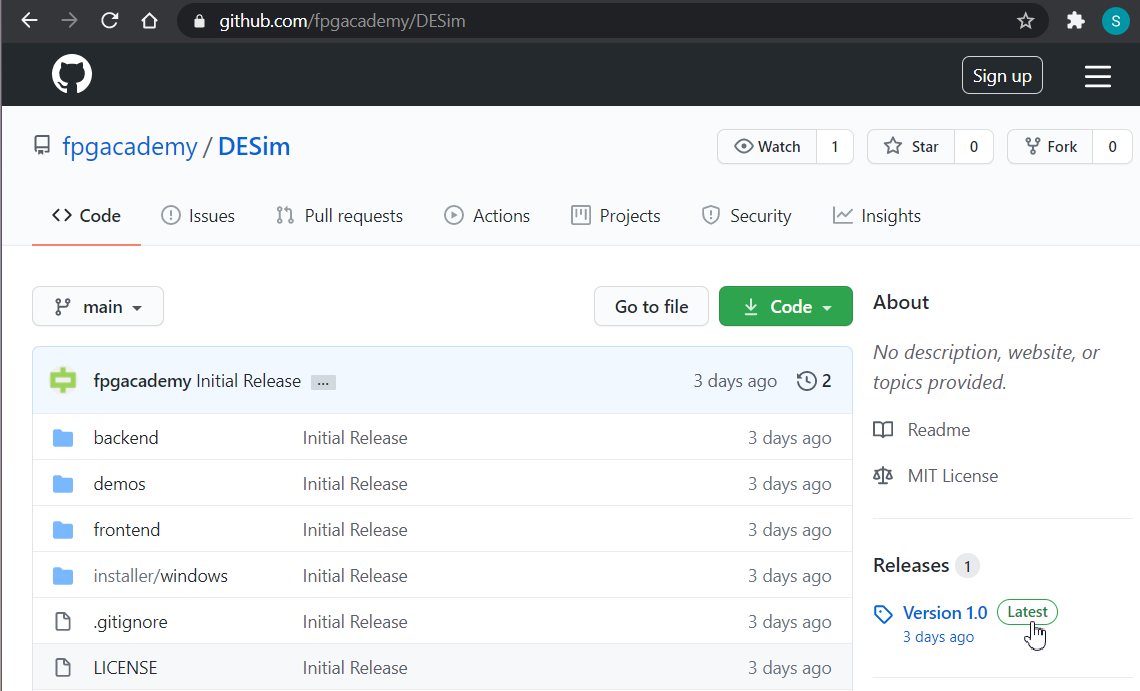
\includegraphics[width = \textwidth]{figures/github.png}}
	\end{center}
          \caption{The {\it DESim} repository on {\it GitHub}.}
	\label{fig:github}
\end{figure}

\newpage
~\\
\noindent
Click on the filename {\it desim\_setup.exe}, as illustrated in Figure~\ref{fig:release},
which downloads this file to your computer. You may be presented with a
warning message in your browser, because the file that you are downloading is an 
{\it executable program}. Make the appropriate selections in your browser to keep the downloaded
file so that it is saved onto your computer.

\begin{figure}[h]
	\begin{center}
        \setlength{\fboxsep}{0pt}
        \fbox{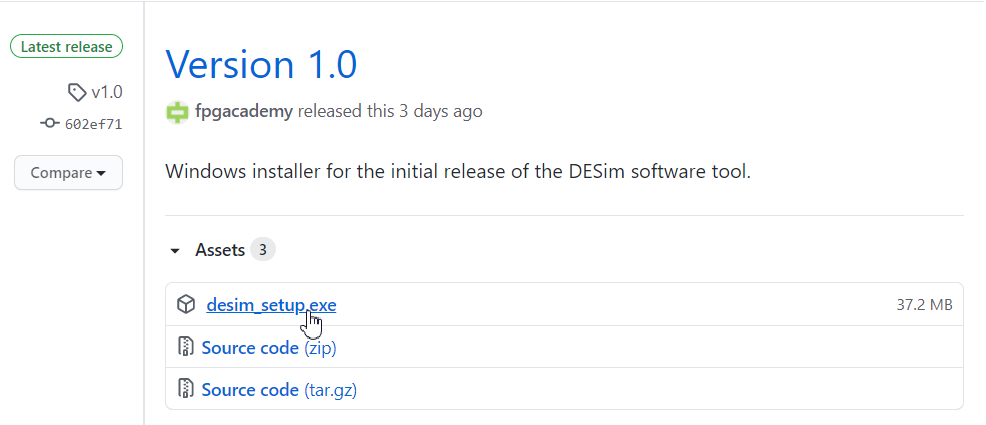
\includegraphics[scale=0.75]{figures/github_installer.png}}
	\end{center}
          \caption{The \texttt{Releases} page for the {\it DESim} repository.}
	\label{fig:release}
\end{figure}

~\\
\noindent
The {\it desim\_setup.exe} file is the {\it installer} program for the {\it DESim}
application. Open this file (execute the program) to reach the \texttt{Welcome} screen 
shown in Figure~\ref{fig:welcome}. Click \texttt{Next} to see the {\it License Agreement}
for the {\it DESim} application, and then click \texttt{I Agree} if you accept the terms of 
the license. If you do not accept the terms of the agreement, then the installer will
exit. Click \texttt{Next} to reach the screen displayed in Figure~\ref{fig:install}.

~\\
\begin{figure}[h]
	\begin{center}
        \setlength{\fboxsep}{0pt}
        \fbox{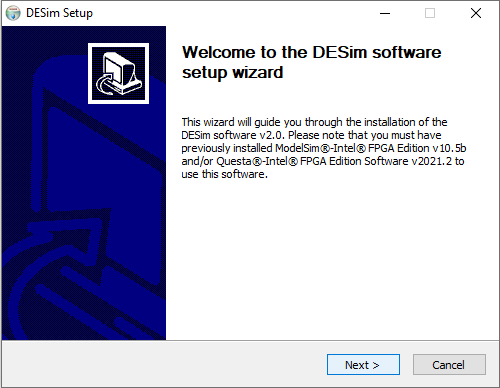
\includegraphics[scale=.75]{figures/welcome.png}}
	\end{center}
          \caption{The first screen of the {\it DESim} installer.}
	\label{fig:welcome}
\end{figure}

\noindent
In Figure~\ref{fig:install} you can specify an installation folder. In the discussion
below we assume that you have accepted the default location (\texttt{C:$\backslash$DESim}),
but you can change this selection. Click the \texttt{Install} button. 
During the installation process you have the option of placing an icon onto your
\texttt{Desktop} for this application. This icon provides an easy way to run the {\it DESim}
application, and so is recommended. 

\begin{figure}[h]
	\begin{center}
        \setlength{\fboxsep}{0pt}
        \fbox{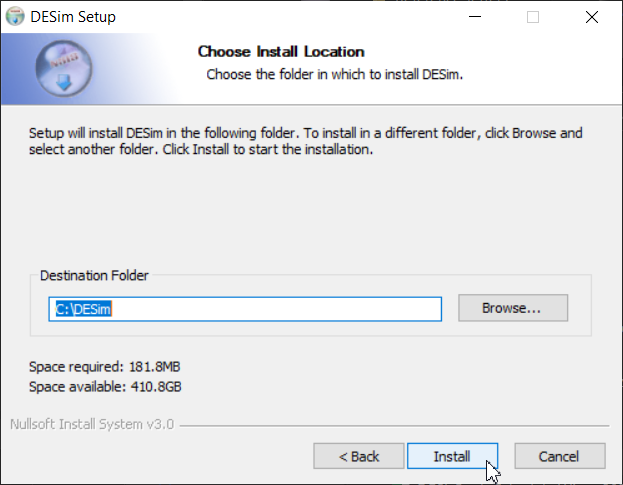
\includegraphics[scale=.75]{figures/install.png}}
	\end{center}
          \caption{Installing the {\it DESim} application.}
	\label{fig:install}
\end{figure}

\noindent
The \texttt{C:$\backslash$DESim} folder created in the installation process
contains the {\it DESim} software and some
example projects (called {\it demos}). Start the {\it DESim} application by double-clicking its
{\it icon} on your \texttt{Desktop}, or by selecting {\it DESim} from the 
{\it Windows Start} menu. Alternatively, you can use \texttt{File Explorer} to run the 
{\it DESim} application by navigating to the \texttt{C:$\backslash$DESim} folder, 
right-clicking on the {\it batch} file \texttt{DESim\_run.bat}, as illustrated in 
Figure~\ref{fig:open}, and then selecting \texttt{Open} (or, you can double-click on the 
batch file to open it). You should now see the {\it DESim} graphical user interface (GUI),
illustrated in Figure~\ref{fig:GUI}. It should show the message
``\green{The server is running...}'' near the top of the {\it message pane} in the GUI.

~\\
\begin{figure}[h]
	\begin{center}
            \setlength{\fboxsep}{0pt}
            \fbox{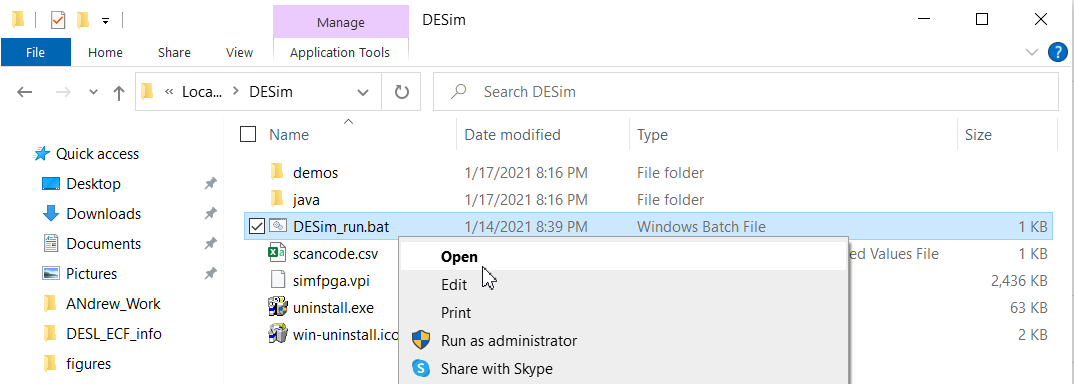
\includegraphics[width = 1\textwidth]{figures/DESim_open_local.png}}
	\end{center}
          \caption{Starting the {\it DESim} application.}
	\label{fig:open}
\end{figure}

\begin{figure}[h]
	\begin{center}
		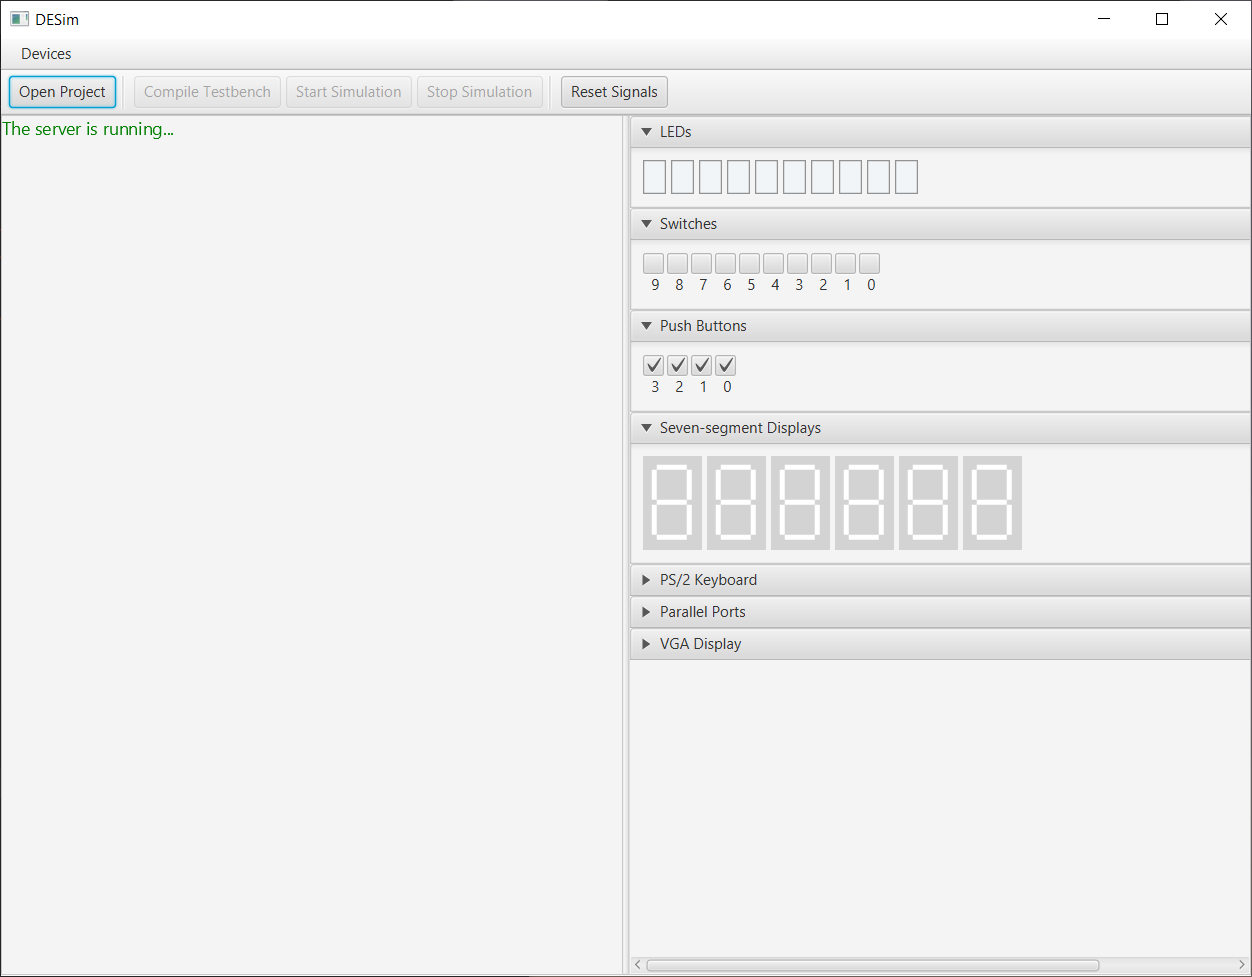
\includegraphics[width = \textwidth]{figures/DESim_GUI.png}
	\end{center}
          \caption{The {\it DESim} window.}
	\label{fig:GUI}
\end{figure}

\noindent
To ensure that the {\it DESim} application can communicate with the {\it ModelSim} simulator, you
may wish to try out one (or more) of the {\it demo} projects that come with {\it DESim}. As
an example, click the \texttt{Open Project} command in the {\it DESim} GUI and then 
navigate into
the \texttt{demos} folder. As illustrated in Figure~\ref{fig:demos}, click to select the 
folder named \texttt{LED\_HEX} and then click on the \fbox{\texttt{Select Folder}} button.

\begin{figure}[h]
	\begin{center}
        \setlength{\fboxsep}{0pt}
        \fbox{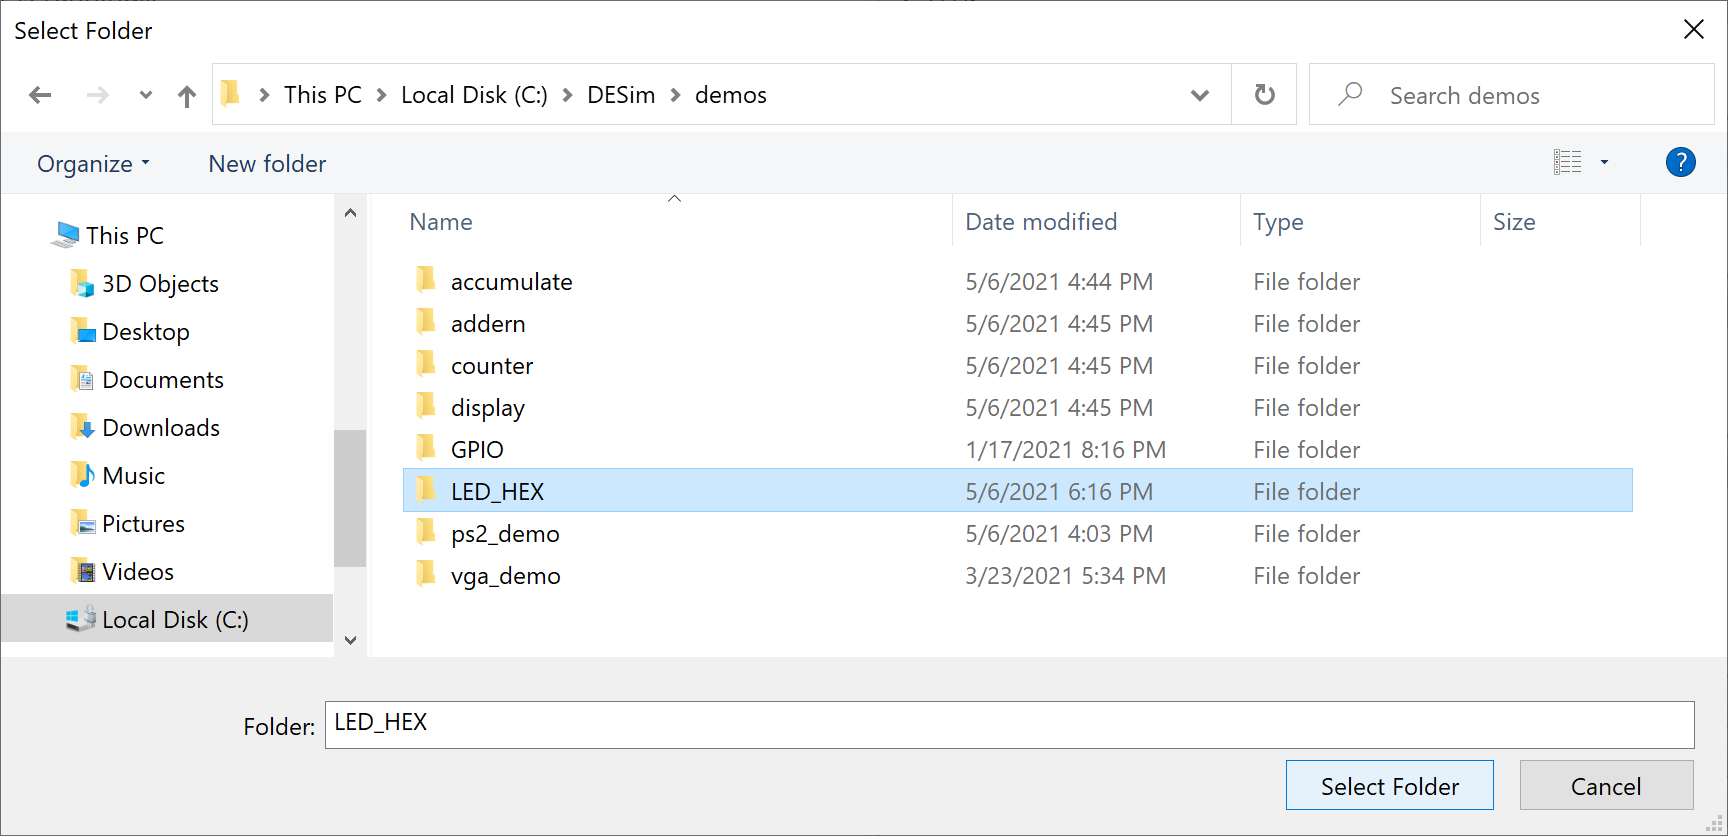
\includegraphics[width = .9\textwidth]{figures/DESim_project.png}}
	\end{center}
          \caption{Opening a sample project in the \texttt{demos} folder.}
	\label{fig:demos}
\end{figure}

~\\
\noindent
Click the \texttt{Compile Testbench} command in {\it DESim}. As shown in 
Figure~\ref{fig:compile}, the ModelSim simulator is executed to compile the Verilog
code for the sample project, and the compilation messages that are produced by 
{\it ModelSim} are displayed in the {\it DESim} message pane.

~\\
\noindent
In the {\it DESim} window select the \texttt{Start Simulation} command, which runs the
ModelSim Verilog simulator. As illustrated in Figure~\ref{fig:sim} any messages produced
by {\it ModelSim} are displayed in the message pane of the {\it DESim} window. To make your
display look like the one in the figure, in the {\it DESim} GUI click on 
the \texttt{Switch} with index number
\texttt{6}, which causes the corresponding \texttt{LED} to turn \red{red}. To activate the
\texttt{Seven-segment Display} output you have to reset the \texttt{LED\_HEX} circuit. To
do this, click on \texttt{Push Button} \texttt{0} to press it, and then click again to
release this button. 
To learn about the features of the \texttt{LED\_HEX} project, you can follow 
the instructions in its {\it Readme.txt} file, shown in Figure~\ref{fig:readme}, and/or 
read through the Verilog source-code file \texttt{LED\_HEX.v}, displayed in 
Figure~\ref{fig:top}. These files can be found
using the Microsoft Windows \texttt{File Explorer} in the \texttt{LED\_HEX} folder.

~\\
\noindent
You can stop the {\it ModelSim} simulation by selecting the \texttt{Stop Simulation}
command in the {\it DESim} GUI. To close the {\it DESim} program click the $\times$ in 
the upper-right corner of the window.    

\begin{figure}[h]
	\begin{center}
        \setlength{\fboxsep}{0pt}
        \fbox{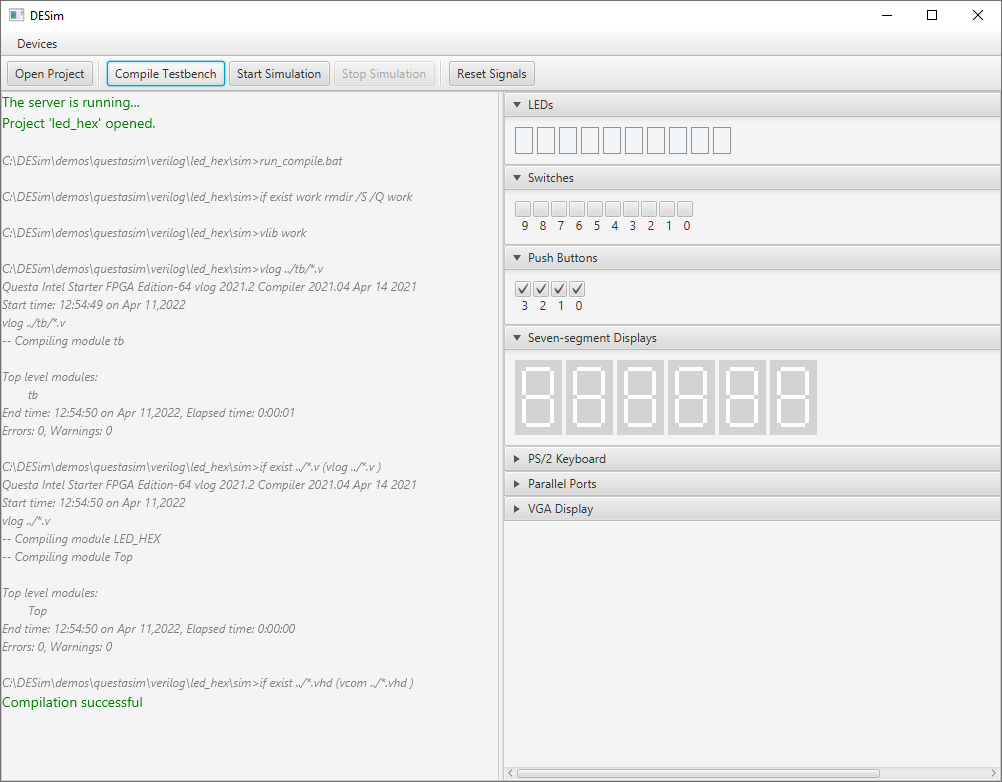
\includegraphics[width = .9\textwidth]{figures/DESim_compile.png}}
	\end{center}
          \caption{Compiling the sample project.}
	\label{fig:compile}
\end{figure}

\begin{figure}[h]
	\begin{center}
        \setlength{\fboxsep}{0pt}
        \fbox{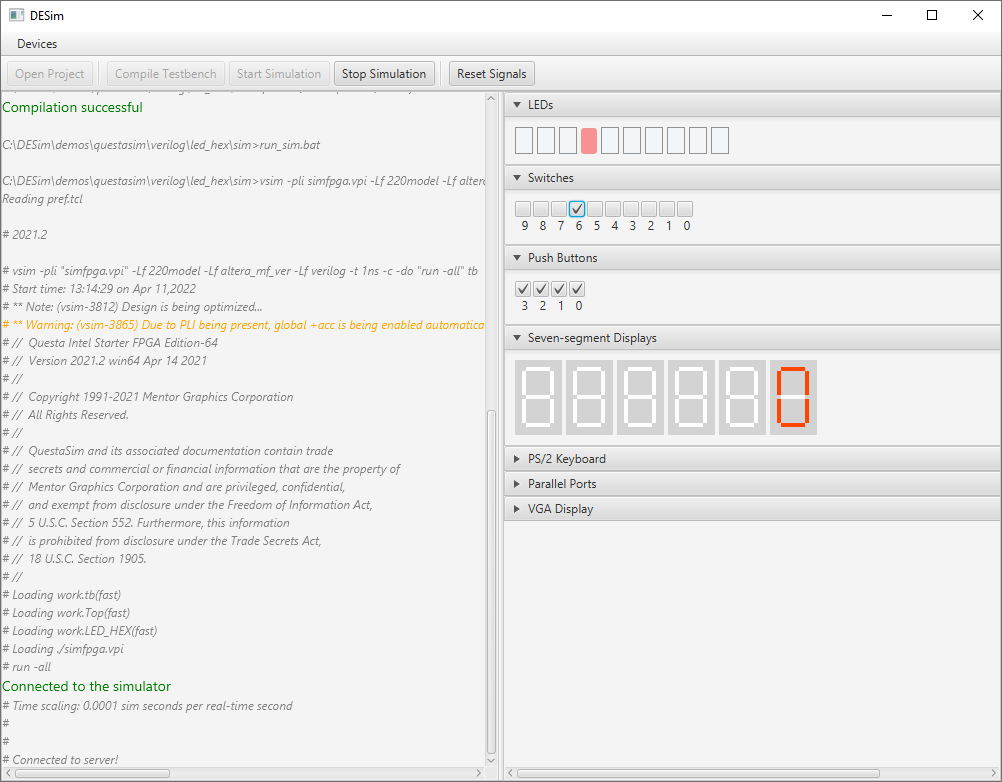
\includegraphics[width = \textwidth]{figures/DESim_simulate.png}}
	\end{center}
          \caption{Simulating the sample project.}
	\label{fig:sim}
\end{figure}

\lstset{language=make,numbers=none,escapechar=|}
\begin{figure}[h]
\begin{center}
\begin{minipage}[t]{12.5 cm}
\begin{lstlisting}[name=readme]
To use this demo:

-- SW are displayed on LEDR
-- KEY[0] is the synchronous reset. It sets the HEX-display selector to 0.
-- KEY[1] provides the active-low enable for the HEX-display selector

To use:
1. First press/release KEY[0] to reset the circuit; HEX0 is selected
   -- HEX0 can be changed using SW[6:0]
2. Set SW[9:7] to select a different HEX display (from 0 to 5) 
   -- press/release KEY[1] to store the selected HEX address
   -- the selected HEX display can now be changed using SW[6:0]
3. Set SW[9:7] to select another display, etc.
\end{lstlisting}
\end{minipage}
    \caption{The {\it Readme.txt} file for the \texttt{LED\_HEX} project.}
\label{fig:readme}
\end{center}
\end{figure}

\lstset{language=Verilog,numbers=none,escapechar=|}
\begin{figure}[h]
\begin{center}
\begin{minipage}[t]{15 cm}
\begin{lstlisting}[name=addern]
module LED_HEX (CLOCK_50, SW, KEY, LEDR, HEX0, HEX1, HEX2, HEX3, HEX4, HEX5);
    input wire CLOCK_50;
    input wire [9:0] SW;
    input wire [1:0] KEY;
    output wire [9:0] LEDR;         // DE-series LEDs   

    output reg [6:0] HEX0;          // DE-series HEX displays
    output reg [6:0] HEX1;
    output reg [6:0] HEX2;
    output reg [6:0] HEX3;
    output reg [6:0] HEX4;
    output reg [6:0] HEX5;

    assign LEDR = SW;

    reg [2:0] Addr;                 // used to select a HEX display

    always @ (posedge CLOCK_50)
        if (KEY[0] == 0)            // sync reset
            Addr <= 3'b0;
        else if (KEY[1] == 0)       // select a HEX display
            Addr <= SW[9:7];

    always @ (posedge CLOCK_50)
        case (Addr)
            3'b000:  HEX0 <= SW[6:0];
            3'b001:  HEX1 <= SW[6:0];
            3'b010:  HEX2 <= SW[6:0];
            3'b011:  HEX3 <= SW[6:0];
            3'b100:  HEX4 <= SW[6:0];
            3'b101:  HEX5 <= SW[6:0];
            default: ;
        endcase

endmodule
\end{lstlisting}
\end{minipage}
        \caption{The Verilog source-code file \texttt{LED\_HEX.v}.}
\label{fig:top}
\end{center}
\end{figure}

\end{document}
